\documentclass[12pt]{article}
\setlength{\oddsidemargin}{0in}
\setlength{\evensidemargin}{0in}
\setlength{\textwidth}{6.5in}
\setlength{\parindent}{0in}
\setlength{\parskip}{\baselineskip}

\usepackage{amsmath,amsfonts,amssymb,graphicx,hyperref,xcolor}

\newcommand{\purple}[1]{{\color{purple} #1}}

\begin{document}

PHYS 374 Fall 2020\hfill Worksheet 3: Shortest Path on a Cylinder and a Sphere\\
\\
Name: \purple{SOLUTION} \\
\\
Please submit as a PDF on Moodle. Include any calculations made using external tools.

\hrulefill
\\
\\
\noindent
\textbf{Part I: }Consider a cylinder of radius $R$. The relationship between quantities in \href{https://mathworld.wolfram.com/CylindricalCoordinates.html}{Cylindrical} and Cartesian coordinates is
\begin{equation}
\begin{split}
x&=\rho\cos\phi\\
y&=\rho\sin\phi\\
z&=z
\end{split}
\end{equation}
\begin{enumerate}
\item Find the infinitesimal path length, $dl$ in cylindrical coordinates noting that the radius $\rho$ is fixed for the surface of a cylinder.
\item Use calculus of variations to find the shortest path on a cylinder with radius $R$ between two arbitrary points $A$ and $B$.
\item What is the shortest path if the starting and ending heights ($z$) are identical?
\item Does your answer in part 2. reduce to the correct answer? Discuss.
\item What is the shortest path if the starting and ending angles ($\phi$) are identical?
\item Does the answer in part 2. reduce to the correct answer?
%\begin{figure}[h]
%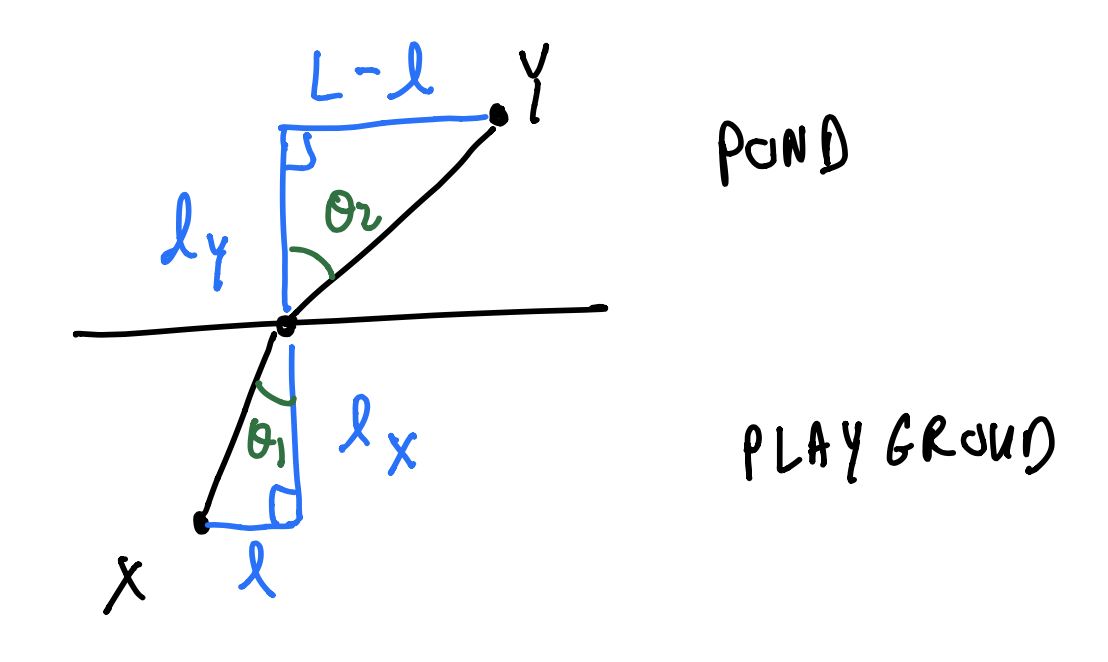
\includegraphics[width=8cm]{Diagram}
%\centering
%\end{figure}
\end{enumerate}
\textbf{Part II: }Consider a sphere of radius $R$. The relationship between quantities in \href{https://mathworld.wolfram.com/SphericalCoordinates.html}{Spherical} and Cartesian coordinates is
\begin{equation}
\begin{split}
x&=r\sin\theta\cos\phi\\
y&=r\sin\theta\sin\phi\\
z&=r\cos\theta
\end{split}
\end{equation}
\begin{enumerate}
\item Find the infinitesimal path length, $dl$ in spherical coordinates noting that the radius $r$ is fixed for the surface of a sphere.
\item Use calculus of variations to find the shortest path on a sphere with radius $R$ between two arbitrary points $A$ and $B$.
\item Discuss limiting cases.
\end{enumerate}

\purple{
\textbf{Part I}

We're looking at the surface of the cylinder -- $\rho$ is constant -- so:
$$
dx = -\rho \sin\phi \, d\phi
\quad \quad
dy = \rho \cos\phi \, d\phi
\quad \quad
dz = dz
$$
So:
$$
d\ell = \sqrt{dx^2 + dy^2 + dz^2} = \sqrt{ \rho^2d\phi^2 + dz^2}
$$
Note we used the trig identity $\sin^2\phi + \cos^2\phi = 1$. The differential length element $\rho d\phi$ corresponds to the horizontal direction (around the cylinder) while $dz$ is up and down. Integrating over a whole path, the length from $A$ to $B$ along the path $z(\phi)$ is:
$$
\ell = \int_{\phi_A}^{\phi_B} d\phi \, \sqrt{ \rho^2 + z'^2 } \quad \quad \mathrm{where} \quad \quad z' = \frac{dz}{d\phi}
$$
The above integral takes the form $\int d\phi \, f(z, z', \phi)$. The corresponding Euler-Lagrange equation is:
$$
\frac{\partial f}{\partial z} - \frac{d}{d\phi} \left( \frac{\partial f}{\partial z'} \right) = 0
$$
Evaluating the derivatives of $f$and plugging them in, we get:
$$
0 - \frac{d}{d\phi} \left( \frac{z'}{\sqrt{\rho^2 + z'^2}} \right) = 0
$$
Recall $\rho$ is constant, so this can be true only if $z'$ is also constant. Call it $m$:
$$
\frac{dz}{d\phi} = m
\quad \rightarrow \quad
dz = m \, d\phi
\quad \rightarrow \quad
z(\phi) = m \, \phi + b
$$
In other words, if we marked the shortest path $z(\phi)$ from $A$ to $B$ on the surface of the cylinder, then ``unrolled" the cylinder onto a flat surface, it would be a straight line. 


If $z_A = z_B$ then the slope $m$ is zero, since the path is a horizontal line with no dependence on $\phi$.

If $\phi_A = \phi_B$, things get dicey. We're talking about more than one value of $z$ for the same value of $\phi$, so the path can't be expressed as a function $z(\phi)$. One thing we can do is use limits. As $\phi_A \rightarrow \phi_B$, the behavior is clear: the slope $m$ becomes increasingly steep, approaching a vertical line. It's clear that in the limiting case, the shortest path is a straight vertical line.

We can also talk about this path by inverting $z(\phi)$ to get $\phi(z)$: 
$$
\phi(z) = \mu \, z + \beta
$$
It's possible to relate $m$ and $b$ to $\mu$ and $\beta$, but it doesn't really tell us anything. They all take whatever values line up with the endpoints $A$ and $B$. 
If $\phi_A = \phi_B$ we can then choose $\mu = 0$ to line up with both endpoints. On the other hand, if we want to use $\phi(z)$ to talk about the case where $z_A = z_B$, we have to use limits.
}


\purple{
\textbf{Part II}

We're looking at the surface of the sphere. Radius is constant, but both $\theta$ and $\phi$ vary. So for each term, we have to use the product rule to look at differential elements in both directions:
$$
dx = -r \sin\theta \, \sin\phi \, d\phi + r \cos\theta \, \cos\phi \, d\theta
\quad
dy = r \sin\theta \, \cos\phi \, d\phi + r \cos\theta \, \sin\phi \, d\theta
\quad
dz = r \sin\theta \, d\theta
$$
So after a fair amount of cancellation:
$$
d\ell = \sqrt{dx^2 + dy^2 + dz^2} = \sqrt{ r^2 d\theta^2 + r^2 \sin^2 \theta d\phi^2}
$$
Note that the $d\theta$ term corresponds to a path length in the north-south direction, while the $d\phi$ term can be thought of as east-west. The $\sin\theta$ is there because lines of latitude are shorter close to the poles. 

Plugging this expression into an integral to get a path from $A$ to $B$ gives:
$$
\ell = \int_{\phi_A}^{\phi_B} d\theta \, r \sqrt{ 1 + \sin^2 \theta \phi'^2 } \quad \quad \mathrm{where} \quad \quad \phi' = \frac{d\phi}{d\theta}
$$
The above integral takes the form $\int d\theta \, f(\phi, \phi', \theta)$. The corresponding Euler-Lagrange equation is:
$$
\frac{\partial f}{\partial \phi} - \frac{d}{d\theta} \left( \frac{\partial f}{\partial \phi'} \right) = 0
$$
Evaluating the derivatives of $f$and plugging them in, we get:
$$
0 - \frac{d}{d\phi} \left( \frac{\sin^2\theta \phi'}{\sqrt{ 1 + \sin^2 \theta \phi'^2 }} \right) = 0
$$
The term in parentheses must be constant. Let's call it $k$:
$$
\frac{\sin^2\theta \phi'}{\sqrt{\cdots}} = k \quad \text{(constant)}
$$
Geometrically, a sphere looks identical regardless of rotation. So without loss of generality, we can rotate the sphere until our starting point $A$ is at the north pole. In that case, $\sin\theta=0$, which in turn means $k=0$.

And if $k=0$, $\phi'=0$ everywhere other than the pole (since $\sin\theta=0$ only at the pole). So $\phi'=0$. In other words, the shortest path from the pole to any other point on a sphere is to follow a line of longitude. 

An analogous argument can be made by rotating the globe until $A$ and $B$ both fall on the equator, then showing that $\frac{d\theta}{d\phi}=0$. 

To generalize back to arbitrary points on a sphere, shortest paths must always fall on a circular path with radius $r$. This is called a ``great circle." 

As a visualization tool, look at airplane flight paths. You don't fly due east from San Francisco to Tokyo, even though the two cities are at the same latitude. It's shorter to fly north over Alaska, then back south. This path can be found by rotating the globe until San Francisco is at the ``top" then drawing a line straight ``down" -- or by rotating it until both cities are at the ``equator" then drawing a line ``horizontally."
}




\end{document}